\begin{figure}[!htb] 
\centering 
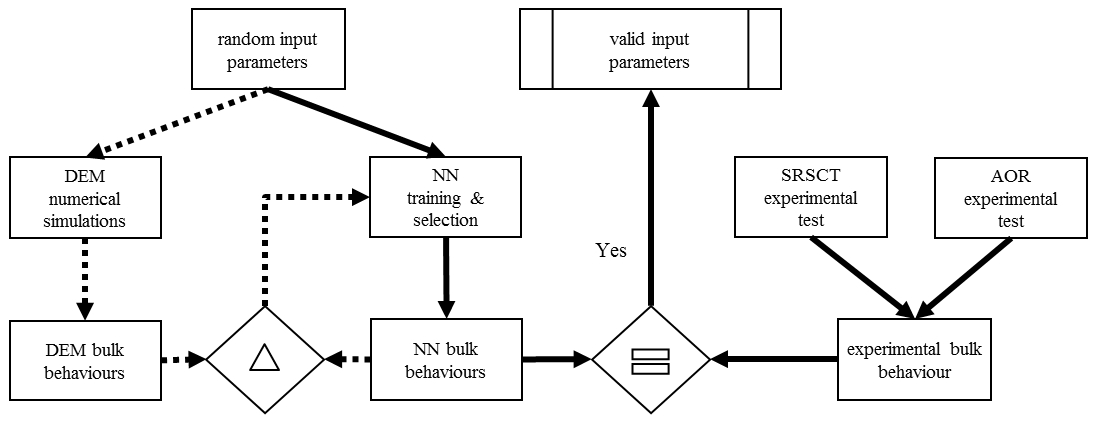
\includegraphics[width=.96\textwidth]{images/19methodology} 
\caption[Method]{Method. 
In the training phase (dashed lines)
$DEM$ simulations are performed
with random initial input parameters.
The behaviours obtained are used to train the
Artificial Neural Networks ($ANNs$) in a loop that continues until the
difference between the outputs of each $ANN$ and its simulations is below the
limit ($\Delta$) (see Section \ref{subsec:ann}).
In the parameters identification phase (solid
lines) we identify valid input parameters by comparing (\textbf{=}) $ANNs$ and
experimental behaviours.
Further explanations can be found in Section \ref{sec:methodology}.
}
\label{fig:19methodology} 
\end{figure}